\chapter{Conclusion}



\section{Closing Discussion}

Discussion on the example

Talk about why I wanted to write this, how the process went, world of possibilities it opened up for further research.

- Perhaps put in the "future work" section the idea of modeling rare events wth Bayes



\section{Further Research}


As by design, this thesis has intended to further the reader's understanding of neural networks by use of the Bayesian paradigm.  It has outlined many preferable traits of BNNs and the functional suitability they have for revealing highly complex trends in data.
This section is devoted to the primary inspirations for further research on Bayesian Neural Networks, based either in theory or application, or both.

\subsection{Model Comparison}
As promised at the beginning of this chapter, Bayes can be applied to select an ideal capacity model \cite{bishop1997bayesian}.  Consider three networks of different capacities (for example, the the three networks from the Tohoku Earthquake MLP example, each with an additional hidden layer).  Now, suppose they are Bayesian networks represented as $A_1, A_2, A_3$ with the subscript representing the number of hidden layers.
$$
p(A|D) = \frac{p(D|A)p(A)}{p(D)}
$$
Without justification to prefer one model over the other, the prior $p(A)$ would be the same.  Therefore, the complexity of the model is contingent only upon the data likelihood under each model $p(D|A)$.  Different models can be compared; the model with the highest likelihood of the data has better evidence for its predictions. Below is an arbitrary representation of these networks.  More complex models fit a wider range of data \cite{bishop1997bayesian}, indicated by the wider curves.  However, these have less likelihood than simpler models for certain data sets; one of which is represented by the red line.

\begin{figure}[H]
    \centering
    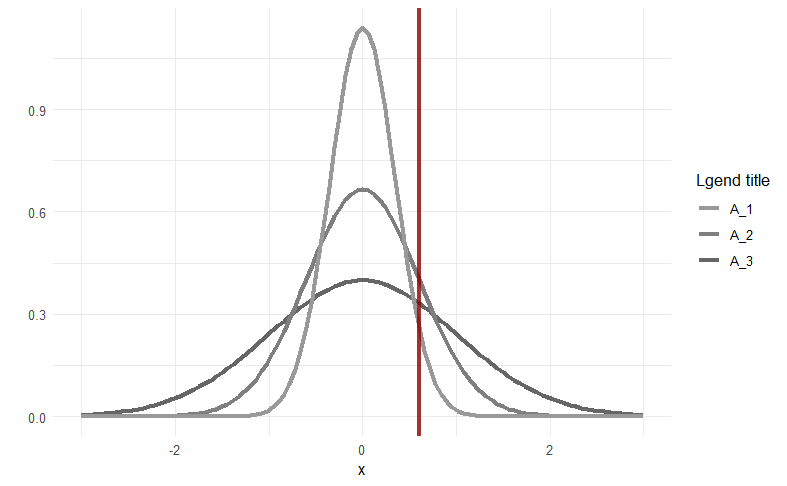
\includegraphics[width = .6\textwidth]{Figures/BNN_modelcheck.png}
    \caption{\footnotesize{Arbitrary representation of network generalizability, based on model complexity controlled by the number of hidden layers. Data within the central tendency of the red line may find the network with two hidden layers to be the most preferable}}
    \label{BNNmodelcheck}
\end{figure}

It would be interesting to compare specific architectures for the Tohoku Earthquake example, or any other appropriate example too.  Moving beyond, the application of Bayes to convolutional layers, specifically a comparison of probabilistic and deterministic models for high-level computer vision tasks, would be worth studying.


\subsection{Online Learning}
One can imagine scenarios in which the data is becoming available in real time, or even situations where a model is trained incrementally on data, as though it was fed through a hopper.  This makes especially interesting Bayesian techniques for online learning \cite{opper1999bayesian}, in which the BNN is trained in this way.  The Bayesian Updating rule would apply to cyclically recycle posteriors into priors in the presence of new data.  Further studies on this concept would be interesting to apply to practical application, such as in stock price fluctuation or weather prediction.

\subsection{BNN/ANN Regularizers}
It was noted several times that the assumptions of the prior distribution directly impact the BNN, specifically the recognizable regularization technique that its point-estimate correspondent would employ.  Literature \cite{vladimirova2019understanding} \cite{chiuso2016regularization} makes note of alternative priors and their coincidence with other regularization techniques (i.e. LASSO).  However, no publication exists based solely on the resemblance of probabilistic models with specific priors and their non-Bayesian counterparts.  It could be noteworthy to compare models built under each paradigm and demonstrate the level of engineering each would require as well as their predictive capabilities.